\subsection{Initial Approach}
\subsubsection{Outline}

The initial solution is to implement a simple MLP neural network which will be trained by raw input data. The intention is to observe the output of the trained network and the network itself and analyse the results to get a sense of direction.\\

\includegraphics[scale=0.55]{initial_approach_outline.png}

\subsubsection{Input Extraction}

The input of the system is pairs of files that compose a DDR game. One of the files is a music file and the other is a steps file. The DDR emulator will parse these 2 files and play the music file in sync with the steps file so the user may play the game.
The music file may come in many different formats such as MP3s, WAVs, AIFFs, and many more. However, all formats are just different representations of raw sound signals and can be readily converted to each other. Some file formats are compressed and will need to be uncompressed. The Wav file format is a standard uncompressed file format. This project converts all input music files to the Wav file format so that only one parser needs to be written. As well, the Wav file format is the easiest to work with because of its very transparent way of data storage.\\

The Wav file format [1] stores a frequency and bitrate followed by a series of sound signals that compose the sounds to be played. The frequency determines the time duration of each sound signal and the bitrate determines how many bits are used to represent each sound signal. The higher these values are, the finer the sound and the more it resembles analog sound. A parser is built to parse a wav file into memory as a list, where each item of the list will represent the amplitude of the sound signal at the time index * (1 / frequency). The wav file may contain more than one channels in which case the resulting list will have one dimension for each channel.
The steps file comes in only one file format (SM file[2]) for the PC emulator. The steps file represent the step data using measures. Each measure will contain data about which arrows will be displayed on the screen at each fraction of the measure (valid fractions are all over powers of 2). The length of each measure is specified in the header of the file, along with other various data that dictate timing factors. A parser is created to parse the steps file into memory as a list, where each item of the list will be a 1 or 0 to represent whether or not a step was present at the exact moment specified by the index. The amount of time each index represents is configurable and will be called with parameters to match that of the sound signal.\\

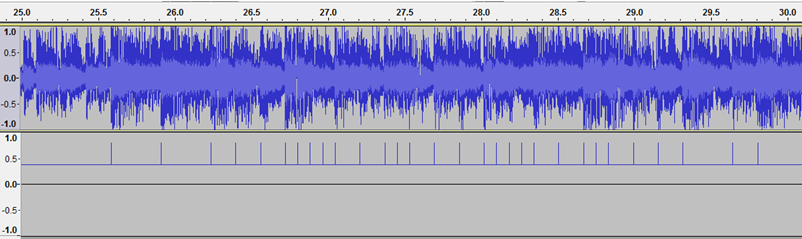
\includegraphics[scale=0.55]{signal_1.png}

Figure x. A visualisation of the sound signal array (top) and the beat signal array (bottom) of a sample input set.


\subsection{Neural Network}
A custom implemented MLP neural network is used to train the data. The configurable parameters are the number of layers, size of each layer, and the input/output size. The neural network is also able to export its current state to file so it can be imported for further training or use.\\

As mentioned previously, the input of the neural network is the raw data of the sound signal and steps signal. A series of sound signals is expected as input and a series of steps signals is expected as output. The entire signal array for both the sound and steps are split up into chunks of 100 signals, and the input/output size of the neural network is configured to 100. For a given song, one epoch consists of running each chunk of 100 signals of the song through the neural network and performing backpropagation.
The algorithm used in the MLP neural network is identical to the backpropagation algorithm discussed in lectures.\\

 At the start of each epoch, each node in the network is initialised with a random weight for each of its parent nodes. When forward propagation of data occurs, the value of the input nodes will be initialised as a chunk of 100 signals of the song. The value of other nodes is then calculated as the summation of the product of each parent node’s value and its respective weight in the current node. The value is then put through a sigmoid activation function before being used by the child nodes. The value of the output nodes is compared to the chunk of 100 signals of the steps. Error is calculated using gradient descent and back propagated. The cumulative error is calculated as the summation of (expected output – actual output) * (1 – output) * (output) across all iterations of the epoch. The weights are updated based on errors and another epoch begins. \\\\
 
 
\subsubsection{Time Analysis and Compromise}
Initial configuration of the neural network resulted in each iteration of the epoch taking around 0.00015 seconds. On average, a song will have 4 million signal samples which will result in around 40000 iterations per epoch after the subdividing the original signal into chunks. The resulting time per epoch is around 10 hours and is way less than reasonable. The parameters of the neural network were toned down to improve runtimes. The size of each layer was reduced by tenfold and so was the number of layers. This resulted in a rough improvement of 1000 times since the backpropagation algorithm was O($n^2$) on the width of the layer and O(n) on the number of layers. The resulting time per epoch was 30 seconds.\\

\subsubsection{Neural Network Training}
The neural network was trained for a single song as an initial test. The observation was that the cumulative error converged at around 1.9 after 400 epochs, from an initial cumulative error of around 400. When other songs were added to the training set, the cumulative error did not increase by a significant amount. As well, the cumulative error still converged at around 1.9. It was decided at this point that the neural network is in a trained state because the cumulative error did not improve upon further epochs. \\

\subsubsection{Results and Analysis}
The neural network implemented in this section experienced premature convergence because the cumulative error did not converge at 0. A music file was inputted into the neural network and its output was observed. The output was observed to contain values between 0.0018 and 0.0026 which meant the neural network decided that there should be no steps for the given music file. This decision was completely unwanted because it is never the case that a music file does not have a single step. As well the max and min of the output array had no observable correlation to either the expected output array or the input array.\\

With the extreme skew of the output, a different approach was used to decide the actual value of the steps output array. The output array from the neural network is used as a probability array. Each element of the array dictates the chance that a step should occur at that time. This probability is further adjusted based on the amount of time that has passed since the last step was detected. This is to account for the fact that steps will never occur too close to each other and that the distance between consecutive steps is always within some threshold.\\\\

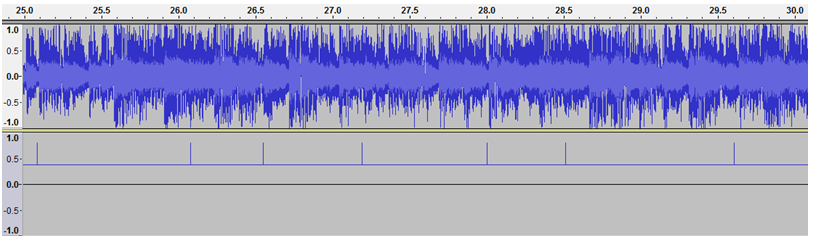
\includegraphics[scale=0.55]{signal_2.png}

Fig x. A visualisation of the input (top) and neural network output with fuzzy logic (bottom).
\\\\
The main reason for the premature convergence of the neural network is the naïve model of input and output that was used. While the sound signal array was well populated, the steps signal array was very sparse. This resulted in an expected output of 0 almost all of the time. As a result, the backpropagation algorithm will try to adjust the network so that the output is as close to 0 as possible to minimize the error. Because the 1s are so sparse, the neural network is unable to retain the learned affected weights from the 1s because they are quickly overwritten by 0s.
Another reason why the training did not go well is because of the nature of the input set. The accompanying steps file for each music file is manually generated by human beings. The human would try their best to assign steps to moments in the song where they perceive a beat or some other musical feature. However, because there is a limit to how fast a person can move their feet in a DDR game, not all beats have steps assigned to them. As a result, the steps file is somewhat of a random subset of the beats of the music file. This randomness in correlation acts to confuse the neural network during training.

\subsection{Fuzzy Logic for Input}

After analysis was done, a different way to extract input was attempted to accommodate the sparsity of the steps array. The steps parser was updated so that it may return an array of fuzzified steps. Instead of representing the precise moment of when a step occurred, a bell curve across 100 consecutive samples is used to represent the step, where the peak of the bell curve is the moment the step occurred.

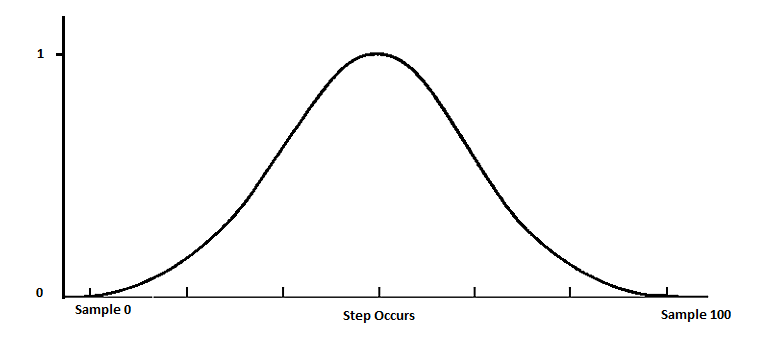
\includegraphics[scale=0.3]{fuzzy.png}

Fig x. Fuzzification of steps in steps array.
This implementation still resulted in premature convergence, with a much larger cumulative error which varies depending on the data set being used. It was conjectured that this methodology is potentially viable perhaps with a different function (instead of a bell curve) with fine-tuned parameters.\\

\subsection{Variable Learning Rate}
Another implementation was attempted to accommodate for the sparsity of the steps array. This implementation allowed the neural network to have a variable learning rate depending on the expected output of the current iteration of the epoch. If the iteration contained an expected of output of 1 in its array, the learning rate is increased to accommodate for the rarity of this expected output. This approach resulted in a trained neural net which gave output with more variance (range 0.0025- 0.0102). However, the output still did not reflect either the expected output or the input array.\\

\subsection{Summary}
The main initial approach had major shortcomings and so did its improved versions. The failures of these approaches can be easily attributed to the naivety of the assumptions made about the data. The overarching idea is that raw data is not what humans use to generate steps file or beats and that they should not be used by machines either because the goal is to simulate human steps generation. A more advanced form of feature extraction is necessary as well as possible other changes to the neural network type and parameters being used.